\documentclass[11pt]{article}
\usepackage[margin=1in]{geometry}
\usepackage{amsmath,amssymb,amsthm,mathtools}
\usepackage{tikz}
\usetikzlibrary{calc,positioning}
\usepackage{listings}
\usepackage[colorlinks=true,linkcolor=blue,citecolor=blue,urlcolor=blue]{hyperref}

\theoremstyle{plain}
\newtheorem{theorem}{Theorem}
\newtheorem{proposition}[theorem]{Proposition}
\newtheorem{lemma}[theorem]{Lemma}
\newtheorem{corollary}[theorem]{Corollary}
\newtheorem{conjecture}[theorem]{Conjecture}
\theoremstyle{definition}
\newtheorem{definition}[theorem]{Definition}
\newtheorem{remark}[theorem]{Remark}
\newtheorem{question}[theorem]{Question}

\newcommand{\enc}[1]{[\![#1]\!]}
\newcommand{\rhoplus}{\rho^{+}}
\newcommand{\bmid}{\mathbin{|}}
\newcommand{\Cell}{\mathsf{Cell}}
\newcommand{\Prime}{\mathsf{Prime}}
\newcommand{\Line}{\mathsf{Line}}
\newcommand{\act}{\mathsf{act}}
\newcommand{\cf}{\mathsf{cf}}
\newcommand{\cc}{\mathsf{cc}}
\newcommand{\pt}{\mathsf{pt}}
\newcommand{\Pasch}{\mathsf{Pasch}}
\newcommand{\PC}{\mathsf{PC}}
\newcommand{\Res}{\mathsf{Res}}
\newcommand{\Sub}{\mathsf{Sub}}
\newcommand{\Desg}{\mathsf{Desg}}
\newcommand{\Conn}{\mathsf{Conn}}

\lstset{basicstyle=\ttfamily\small,columns=fullflexible,breaklines=true,
        showstringspaces=false,frame=none}

\title{Classifying Finite Geometries with a Generated Spatial--Behavioural Logic\\
\large A point is a conflict}
\author{L.\,G. Meredith\\ \small F1R3FLY.io}
\date{July 2026}

\begin{document}
\maketitle

\begin{abstract}
A companion note encodes Batten's near-linear spaces as processes in a mixed-summation
variant $\rhoplus$ of the reflective higher-order calculus, taking the organising decision that a
point is given no term at all and exists only as the set of communications the lines through it
make possible. This note asks what the logic generated from $\rhoplus$ says about those terms.
The programme is a structural analogy with the knot case and not a reuse of it: there,
rho hosts knot diagrams and the generated logic classifies them; here, $\rhoplus$ hosts
geometries and the logic generated from $\rhoplus$ is asked to classify those, on its own terms,
with the knot results carried over nowhere.
The analogy turns out to be an inverting one at almost every joint. Closing a knot destroys the
behavioural layer and leaves the whole discriminating burden to the spatial one; a geometry never
closes, so both layers are live. The knot encoding is conflict-free and hence proof-irrelevant; a
geometry is an object every one of whose points is a race, and that race is the geometry. Knot
formulae are properties of diagrams and descend to knots only through a quotient; geometric
formulae are already properties of the object. And persistence, which the knot encoding needed in
order to be functorial, here \emph{hides} what we want to see, so the classifier reads the
one-shot skeleton rather than the standing form.
The central observation is a single pair of one-line formulae. Two channels are at the same point
exactly when firing one disables the other, and at different points exactly when it does not. So a
point --- the thing deliberately left without a term --- comes back as a connected component of a
behaviourally defined conflict relation, while the number of points on a line is a purely
structural count of parallel components. Batten's two basic numerics therefore sit on two
different layers of the generated logic, and his duality exchanges them.
We take one specification decision (no logical analogue of sums), make one small refinement to the
encoding (a private token per line), and then work a stable of examples: disconnection, the
connection number and Batten's five classes, subplanes, resolvability, and Desargues. We close
with a computation that is small enough to run and can come out either way.
\end{abstract}

\tableofcontents

\section{Introduction}

\subsection{The analogy, stated precisely}

Three notes precede this one. The first \cite{Knots} encodes knot diagrams as cost-accounted
rholang processes and proves the encoding invariant under the Reidemeister moves up to weak
bisimulation. The second \cite{Classifier} observes that because the host is a graph-structured
lambda theory, it comes with a logic generated from its own constructors and rewrite rules by the
OSLF family of algorithms \cite{OSLF}, and that this generated logic already says the things a
knot theorist wants said. The third \cite{Geometry} makes the corresponding move for incidence
geometry: it encodes Batten's near-linear spaces \cite{Batten} in a mixed-summation variant of the
rho calculus, taking the organising decision that a point is not a term but a set of redexes.

The present note stands to \cite{Geometry} as \cite{Classifier} stands to \cite{Knots}. The
relation between the four is a structural analogy:
\begin{align*}
\text{rho} : \text{knots} \;&::\; \text{generated logic} : \text{knot classifiers}\\
:::\qquad \rhoplus : \text{geometries} \;&::\; \text{generated logic} : \text{geometry classifiers}.
\end{align*}
It is worth being explicit about what this does \emph{not} mean, because the temptation is real and
the result of yielding to it would be a much weaker note. We are not carrying the knot classifier's
formulae over to geometry, not asking the knot logic to do double duty, and not treating the
geometric case as a second application of a fixed instrument. The logic generated from $\rhoplus$
is a different logic from the one generated from core rholang, because $\rhoplus$ is a different
theory; and the question we are asking is what \emph{that} logic says about geometries when
nothing is imported to help it.

The answer is more interesting than a transposition would have been, because at nearly every joint
the analogy inverts.

\subsection{Seven ways this is not the knot case}
\label{sec:seven}

We list the differences at once, since they organise everything below.

\paragraph{1. The behavioural layer is alive.}
Closing a knot restricts every arc name, so the encoding of a closed diagram is a live, periodic
$\tau$-network with no free names; weak bisimulation abstracts exactly the internal steps, and the
closed term is nearly featureless as an observable object \cite[\S10]{Knots}. The whole of
\cite{Classifier} is therefore a rescue operation carried out by the spatial layer. A geometry has
no closure step. Its points are its observables and they stay observable \cite[\S8]{Geometry}. Both
layers are live here, and much of what follows is a matter of deciding which one is speaking.

\paragraph{2. There is genuine conflict.}
The knot encoding is a marked graph: every arc is the output port of exactly one gate and the input
port of exactly one \cite[Prop.~1]{Knots}, which is conflict-freedom, which is why liveness,
conservation and periodicity come as cheaply as they do there. It is therefore proof-irrelevant in
the sense of \cite{Choice}: it has no scheduler-side content anywhere. A geometry under the recipe
of \cite{Geometry} is the opposite extreme, an object every one of whose points is a nontrivial
race \cite[Rem.~18]{Geometry}. The races are not noise around the geometry; as \S\ref{sec:point}
argues, they \emph{are} the geometry.

\paragraph{3. There is no quotient to take.}
Almost every formula of \cite{Classifier} is a predicate on diagrams, and the passage from
diagram to knot is a quotient left as downstream work \cite[\S5]{Classifier}. Nothing of the sort
arises here. A near-linear space is its incidence structure; there is no presentation standing
between the object and the term. We return to this in \S\ref{sec:noquotient}, because it is the
single largest structural advantage the geometric case has.

\paragraph{4. The residual gauge is different, and milder.}
What the knot encoding has that is intrinsic --- the crossing sign, fixed by the orientation the
Dowker--Thistlethwaite traversal supplies --- has no counterpart here. What we have instead is the
send/receive polarity of \cite[\S5]{Geometry}, which is a gauge choice and not data. So a formula
must be checked for invariance under re-orientation before a separation it certifies means
anything. This is a discipline the knot note did not need; \S\ref{sec:gauge} supplies it.

\paragraph{5. Persistence hides what we want to see.}
This is the sharpest inversion and we did not expect it. In the knot case reinstatement is what
makes the encoding functorial at all: a forwarder good for one passage would land the encoding in
single-use processes, where composition is not usefully associative \cite[Rem.~5]{Knots}. In the
geometric case reinstatement restores each cell after it fires, and in doing so it erases exactly
the mutual exclusion that carries the incidence data. The classifier therefore reads the grade-0
skeleton of \cite[\S7]{Geometry}, not the standing form. See \S\ref{sec:grade}.

\paragraph{6. There is no cost, hence no ledger cross-check.}
Cost accounting is absent from \cite{Geometry} by design, and we keep it absent. The knot note's
most persuasive small demonstration --- the writhe computed twice, once by running the process and
summing signed debits and once by inspecting the term without running it, with the two required to
agree \cite[\S4.5]{Classifier} --- has no counterpart available to us. We supply a different
two-route demonstration in \S\ref{sec:resolvable}, on the two layers of the logic rather than on
ledger versus logic.

\paragraph{7. The atoms are flags, not crossings.}
A knot term is a flat parallel composition of gates, one per crossing, and the gate is the unit the
characteristic formula describes. A geometry term is a flat parallel composition of one component
per \emph{incident point--line pair}. The line grouping is not recoverable from a flat,
associative--commutative parallel composition, so the encoding needs one small refinement before
the logic can speak about lines at all. That refinement is \S\ref{sec:token}, and it is the one
place where the classifier feeds back into the encoding --- as the greatest fixed point did for
knots \cite[\S2.3.1]{Classifier}.

\subsection{Ideal logic, checkable fragment}

We keep the methodological commitment of \cite[\S1.3]{Classifier} without restating its defence.
The ideal logic is adequate for the idealised calculus and is what defines the invariant; a
fragment, restricted so that model checking terminates, is what decides it; these are different
artifacts with different jobs. The precedent is the Kauffman bracket, defined by a sum over $2^n$
resolutions and computed by something faster. We flag which side of the line each example falls on
as we go, and collect the accounting in \S\ref{sec:check}.

\section{The encoding, with one refinement}

\subsection{Recollection}

We recall only what we use; \cite{Geometry} is the reference. A near-linear space is a pair
$S=(P,L)$ with $L$ a set of subsets of $P$ such that any line has at least two points (NL1) and two
points are on at most one line (NL2). Write $v(\ell)$ for the number of points on $\ell$ and $b(p)$
for the number of lines on $p$. The recipe has four parts:
\begin{enumerate}
\item lines are processes, and the geometry is their parallel composition;
\item points are not terms, but sets of redexes;
\item a line is a parallel composition of one component per incident point, each component a sum
      with one summand per other line through that point;
\item channels are named by pairs of lines: for $\ell_i \neq \ell_j$, the channel $x_{ij}$ sits at
      their common point.
\end{enumerate}
Part 4 is well defined precisely because of NL2 \cite[Prop.~5]{Geometry}: an unordered pair of
distinct lines determines at most one point, hence at most one channel. The base axiom system is
not something the encoding enforces; it is the precondition for the encoding to be definable.

The calculus is $\rhoplus$, core rholang with mixed summation \cite[Def.~9]{Geometry}: summands may
be asynchronous sends as well as receipts, and firing a summand consumes the whole sum. Mixed
summation is forced rather than convenient --- at a point on $k \geq 3$ lines no orientation of the
pairwise channels makes every line's local offer homogeneous \cite[Prop.~7]{Geometry}.

\subsection{Cells}

Call an incident pair $(\ell,p)$ a \emph{flag}, and write $C_{\ell,p}$ for the component the recipe
assigns to it. So
\[
\enc{\ell_i} \;=\; \prod_{p \in \ell_i} C_{i,p},
\qquad
C_{i,p} \;=\; \sum_{\ell_j \ni p,\; j \neq i} \alpha_{ij},
\]
where each $\alpha_{ij}$ is either $x_{ij}!(Q_{ij})$ or $\mathsf{for}(y \leftarrow x_{ij})\{P_{ij}\}$
according to the orientation, and
\[
\enc{S} \;=\; \prod_{\ell \in L} \enc{\ell}.
\]
We call $C_{i,p}$ a \emph{cell}. A cell is the atom of the spatial decomposition: it contains no
parallel composition, so it is $|$-prime.

\begin{remark}[A terminological trap]
In incidence geometry \emph{concurrent} lines are lines through a common point. In process algebra
concurrency is parallel composition. Under this encoding the two senses are opposite: two
incidences of a line at \emph{different} points are in parallel, and two incidences at the
\emph{same} point are in conflict. We therefore avoid ``concurrent'' entirely below and say
\emph{copunctal} for lines through a common point.
\end{remark}

\subsection{The line token}
\label{sec:token}

Parallel composition is associative and commutative, so $\enc{S}$ is a flat parallel composition of
$\sum_{\ell} v(\ell)$ cells --- one per flag --- and nothing in the term records which cells belong
to which line. For the knot encoding this problem does not arise, because a gate is a single term
with its own private latch and the diagram is a flat composition of $n$ gates. Here the flag
decomposition is finer than the line decomposition, and the logic cannot recover the coarser one
from $|$ alone.

The remedy is the one the gate already exhibits. Give each line a private name:
\[
\enc{\ell_i} \;=\; \mathsf{new}\; s_i \;\mathsf{in}\; \Bigl\{ \prod_{p \in \ell_i} C_{i,p}(s_i) \Bigr\}.
\]
The token need not be inert: in the standing form of \cite[\S7]{Geometry} each cell reinstates
itself, and $s_i$ is exactly the channel at which line $\ell_i$'s components are instantiated, so
the refinement costs nothing that the grade-1 form was not already paying. Its effect on the logic
is that the hidden-name quantifier
\[
P \models \mathcal{H}x.\,\varphi \iff P \equiv \mathsf{new}\;x\;\mathsf{in}\;Q \text{ with }
Q \models \varphi, \; x \text{ fresh}
\]
now recovers the line boundary, and $\enc{S}$ becomes a flat parallel composition of $|L|$
line-terms rather than of $\sum_\ell v(\ell)$ cells. This restores the exact structural situation of
the knot case one level up.

\begin{remark}[The classifier amending the encoding]
This is the second instance of a pattern worth naming. In \cite{Classifier} the need for a
characteristic formula of the gate forced a greatest fixed point into the logic. Here the need to
speak about lines forces a private name into the encoding. In both cases the requirement is
independent of the application --- a private token per component is the normal way to make a
composite term addressable --- and in both cases it was invisible until a logic was asked to
describe the term.
\end{remark}

\subsection{Grade 0, not grade 1}
\label{sec:grade}

\cite[\S7]{Geometry} distinguishes three grades: the bare skeleton, whose summands are linear and
which is spent by one passage; the standing geometry, which reinstates itself; and the evolving
geometry, whose continuations compute a successor space. For composability one wants grade 1, for
the same reason the knot gates had to be recursive.

For classification one wants grade 0, and the reason is worth stating carefully because it is
counter-intuitive. Consider a point $p$ on lines $\ell_i,\ell_j,\ell_k$. At grade 0 the firing of
$x_{ij}$ consumes the cells $C_{i,p}$ and $C_{j,p}$ outright, so the redexes $x_{ik}$ and $x_{jk}$
become permanently unavailable: the mutual exclusion at $p$ is starkly observable. At grade 1 both
cells reinstate, and since unfolding a definition is an equation rather than a rewrite
\cite[Rem.~1]{Knots}, the reinstatement is immediate up to structural congruence. The marking
returns, and an observer sees only that a step at $x_{ij}$ was possible --- not that it excluded
anything.

So persistence, which the knot encoding needed, here erases the datum we are trying to read. We
take grade 0 throughout.

\begin{remark}[The other route]
There is a second way out and we record it rather than take it. The adequacy target of a generated
logic is a function of the rewrites: interleaving rewrites yield a logic that sees only
interleaving, true-concurrency rewrites yield a logic that sees true concurrency. Under a step
semantics, mutual exclusion at a point is visible even at grade 1, as the fact that two redexes
cannot fire in one step. That is the right long-run answer, since it lets the classifier read the
composable form of a geometry, but it changes the generated modalities and we do not develop it
here. See \S\ref{sec:open}.
\end{remark}

\section{The logic, as specified}

\subsection{What the generator emits}

Feeding $(\Sigma,E,R)$ for $\rhoplus$ to the generator yields the usual layers \cite{OSLF,Zeus}.

\paragraph{Structural.}
One type former per term former of $\Sigma$. We use $0^\sharp$; the hidden-name quantifier
$\mathcal{H}x.\varphi$ arising from restriction; and, because parallel composition carries an
associative--commutative equational theory, the connective it generates is a genuine separating
conjunction in the sense of \cite{CairesCardelli,Reynolds}:
\[
P \models \varphi \bmid \psi \iff P \equiv Q \bmid R \text{ with } Q \models \varphi,\; R \models \psi.
\]

\paragraph{Behavioural.}
One primitive modality per rewrite rule and choice of redex position, labelled by the one-hole
context in which the step fires rather than merely by an action name. We write $\langle x \rangle
\varphi$ for the modality whose context is a communication at the channel $x$, and take its dual
$[x]\varphi$ as usual. Because $\rhoplus$'s communication rule carries the discard of alternatives,
the context of a step records what was refused as well as what fired.

\paragraph{Propositional and collection.}
Conjunction and $\top$ come from the finite-limits fragment; disjunction and negation require more
and a specification supplies them or does not. We assume all three in the ideal logic. The
collection component is where aggregation lives, and hence where fixed points and counting are paid
for \cite{Zeus}.

\subsection{A specification decision: no connective for sums}
\label{sec:nosums}

The generator emits a structural connective per term former, and $\rhoplus$ has a sum former. We
decline it. The target logic of an OSLF instance is a specification and not a fixed output, so
this is a decision available to us rather than a compromise, and we make it for two reasons.

The expedient reason is that the interaction between a structural presentation of sum syntax and
the behavioural modalities --- which is to say, what structural discrimination of choice buys over
and above what the modalities already give behaviourally --- is a deep question and a large one.
It is flagged in \S\ref{sec:open} and not opened here.

The principled reason is that in this application the connective would describe a distinction the
subject matter does not make. A pencil is a flat unordered set: Batten's lines are sets of points,
there is no nesting and no order among the lines through a point, and the sum at a cell carries no
information beyond its support. A structural connective for $\Sigma$ would let the logic
distinguish presentations of a pencil that the geometry regards as identical.

\begin{remark}[What survives the decision]
One would reasonably worry that declining the sum connective costs us the pencil, and with it
$b(p)$, on which Batten's entire stratification depends. It does not, and the reason is
\S\ref{sec:seven}(2). The discard rule makes conflict \emph{behaviourally} observable, so what the
structural layer is no longer allowed to say, the modalities say instead. This is the first place
where the two layers of the generated logic visibly divide the work, and it sets the pattern for
everything below.
\end{remark}

The resulting architecture is worth stating as a slogan, because it is the shape of the whole note:
\begin{quote}
\emph{The parallel structure of the term is spatial; what a point offers is behavioural.}
\end{quote}
The logic sees which lines there are and which of them meet, structurally; it sees what happens at a
point only through what can fire there.

\subsection{Derived apparatus}

We fix abbreviations used throughout.

\begin{definition}[Primality and counting]
$\Prime := \neg 0^\sharp \wedge \neg(\neg 0^\sharp \bmid \neg 0^\sharp)$ holds of terms with no
proper parallel decomposition. Write $\varphi^{\bmid m}$ for the $m$-fold separating conjunction of
$\varphi$ with itself, and
\[
E_m(\varphi) \;:=\; (\varphi \wedge \Prime)^{\bmid m} \;\wedge\;
\neg\bigl( (\varphi \wedge \Prime)^{\bmid (m+1)} \bmid \top \bigr)
\]
for ``decomposes into exactly $m$ prime parts, each satisfying $\varphi$''. $E_m$ is a
collection-layer device: for a fixed finite space it is a finite formula, and a uniform version
over all spaces requires a fixed point, exactly as alternation did in \cite[Rem.~4]{Classifier}.
\end{definition}

\begin{definition}[Cells, lines, activity]
$\Cell := \Prime$, understood as applying under a line binder.
$\Line := \mathcal{H}s.\, \bigvee_{m \geq 2} E_m(\Cell)$, so that $\enc{S} \models \Line^{\bmid |L|}$.
For a channel $x$, $\act(x) := \langle x \rangle \top$.
\end{definition}

Note what $\act$ is doing. Since the sum connective is unavailable, the only handle we have on a
cell is what it can do, and $\act(x)$ says the cell offers a branch at $x$. The support of a cell
--- the set of channels at which it can act --- is thus a behavioural notion, and it is the
behavioural shadow of the pencil.

\subsection{Gauge: polarity is not data}
\label{sec:gauge}

The transitive orientation fixed in \cite[\S5]{Geometry} --- at a point on $\ell_i,\ell_j,\ell_k$
with $i<j<k$, direct each channel from the higher index to the lower --- is one tournament among
many, and the geometry does not choose it. So a formula that separates two spaces may be separating
two orientations, and a claimed separation is worthless until this is excluded. The knot case has
no analogue of this hazard, since the crossing sign is intrinsic.

The discipline is straightforward once stated. A formula is \emph{gauge-invariant} if its truth
value at $\enc{S}$ is independent of the tournament chosen at each point. Each layer has a
sufficient syntactic condition:
\begin{itemize}
\item name predicates are automatically invariant, since $x_{ij}$ is the same channel whichever way
      it is oriented;
\item a behavioural formula is invariant if it mentions only \emph{which} channel fired and not
      which participant sent --- that is, if it uses $\langle x \rangle$ and not the finer modality
      recording polarity;
\item a structural formula is invariant if it survives the relaxation that forgets polarity, in
      the sense of the relaxation lattice of \cite[\S3.3]{Classifier}.
\end{itemize}
Every formula written below is gauge-invariant by inspection, and we note the point once here
rather than at each example.

\section{A point is a conflict}
\label{sec:point}

This section is the technical heart, and everything in \S\ref{sec:stable} is an application of it.

\subsection{Two one-line formulae}

The organising decision of \cite{Geometry} is that a point receives no term. It follows that if the
logic is to say anything geometric at all, the point must be recovered from something else. It is
recovered from conflict.

\begin{definition}[Conflict and independence]
For channels $x,y$,
\[
x \cf y \;:=\; \act(x) \wedge \act(y) \wedge \langle x \rangle \neg \act(y),
\qquad
x \parallel y \;:=\; \act(x) \wedge \act(y) \wedge \langle x \rangle \act(y).
\]
\end{definition}

\begin{proposition}[Conflict is cell-sharing]
\label{prop:conflict}
At grade 0, $\enc{S} \models x_{ij} \cf x_{kl}$ if and only if the two channels are consumed from a
common cell, i.e.\ $\{i,j\} \cap \{k,l\} \neq \emptyset$ and the two channels sit at the same point.
\end{proposition}

\begin{proof}
Firing at $x_{ij}$ consumes the whole sums $C_{i,p}$ and $C_{j,p}$, where $p$ is the point
$\ell_i \cap \ell_j$. A channel $x_{kl}$ is thereafter unavailable exactly when one of its two
offering cells has been consumed, i.e.\ when $\{k,l\}$ meets $\{i,j\}$ --- say $k=i$ --- and
$C_{i,p}$ is the cell offering $x_{kl}$, which is to say $x_{il}$ sits at $p$. Conversely if the
channels share no cell, both offering cells of $x_{kl}$ survive.
\end{proof}

\begin{corollary}[Copunctal versus triangular]
\label{cor:tri}
Let $\ell_i,\ell_j,\ell_k$ be three pairwise meeting lines. They are copunctal if and only if
$x_{ij}$, $x_{ik}$, $x_{jk}$ are pairwise in conflict, and form a triangle if and only if they are
pairwise independent.
\end{corollary}

This is the distinction Figure~\ref{fig:pencil} draws, and it is the one on which incidence
geometry turns: Desargues, Pappus and Fano are all assertions that certain triples are forced to be
copunctal or collinear, and the whole difference between geometry and the topology of
\cite{Knots} is that these coincidences may not be perturbed away \cite[\S1]{Geometry}. In the
term, the difference between a pencil and a triangle is the difference between one cell offering
two branches and two cells sitting in parallel --- that is, between conflict and parallel
composition, the two most primitive notions the calculus has.

\begin{figure}[t]
\centering
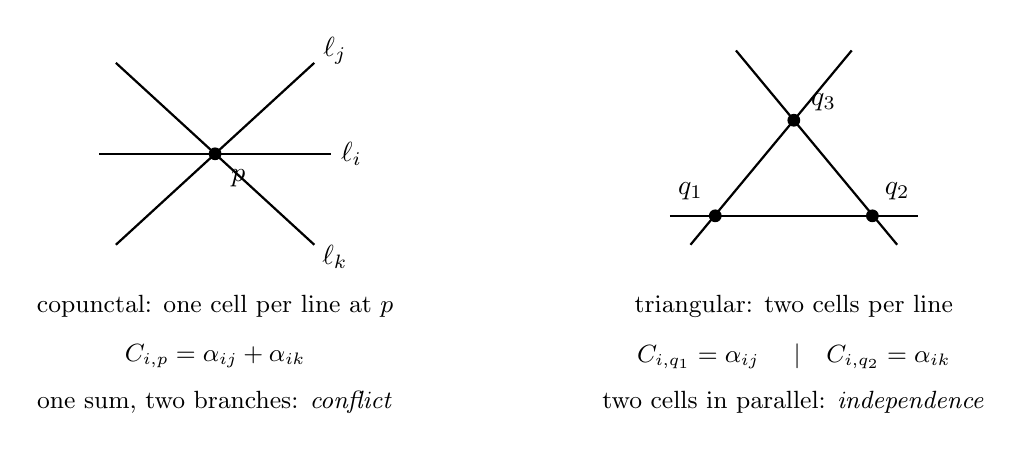
\begin{tikzpicture}[scale=1.05]
% pencil
\begin{scope}
  \draw[thick] (-1.4,0) -- (1.4,0);
  \draw[thick] (-1.2,-1.1) -- (1.2,1.1);
  \draw[thick] (-1.2,1.1) -- (1.2,-1.1);
  \fill (0,0) circle (2.2pt);
  \node at (0.28,-0.3) {$p$};
  \node at (1.65,0) {$\ell_i$};
  \node at (1.45,1.25) {$\ell_j$};
  \node at (1.45,-1.25) {$\ell_k$};
  \node at (0,-1.85) {\small copunctal: one cell per line at $p$};
  \node at (0,-2.45) {\small $C_{i,p} = \alpha_{ij} + \alpha_{ik}$};
  \node at (0,-3.0) {\small one sum, two branches: \emph{conflict}};
\end{scope}
% triangle
\begin{scope}[xshift=7cm]
  \draw[thick] (-1.5,-0.75) -- (1.5,-0.75);
  \draw[thick] (-1.25,-1.1) -- (0.7,1.25);
  \draw[thick] (1.25,-1.1) -- (-0.7,1.25);
  \fill (-0.95,-0.75) circle (2.2pt);
  \fill (0.95,-0.75) circle (2.2pt);
  \fill (0,0.406) circle (2.2pt);
  \node at (-1.25,-0.45) {$q_1$};
  \node at (1.25,-0.45) {$q_2$};
  \node at (0.36,0.62) {$q_3$};
  \node at (0,-1.85) {\small triangular: two cells per line};
  \node at (0,-2.45) {\small $C_{i,q_1} = \alpha_{ij}$ \quad$\bmid$\quad $C_{i,q_2} = \alpha_{ik}$};
  \node at (0,-3.0) {\small two cells in parallel: \emph{independence}};
\end{scope}
\end{tikzpicture}
\caption{Three pairwise meeting lines, the two cases. On the left they are copunctal and each
line contributes a single cell at $p$ offering two branches; firing one branch destroys the other,
so the three channels are pairwise in conflict. On the right they form a triangle and each line
contributes two cells sitting in parallel; the three channels are pairwise independent. The
geometric distinction and the process-algebraic one coincide exactly
(Corollary~\ref{cor:tri}).}
\label{fig:pencil}
\end{figure}

\subsection{Recovering the point}

Conflict is symmetric but not transitive. If $\ell_i,\ell_j,\ell_k,\ell_l$ are all copunctal at $p$
then $x_{ij}$ and $x_{kl}$ share no cell, so they are independent even though they sit at the same
point --- indeed they may fire together, which is exactly the statement that a point on four lines
admits two simultaneous pairings. The relation ``sits at the same point'' is therefore the
transitive closure of conflict.

\begin{definition}[Points as conflict classes]
Let $\pt$ be the least relation with $x \cf y \Rightarrow x \mathrel{\pt} y$ and closed under
transitivity: writing it as a least fixed point,
\[
x \mathrel{\pt} y \;:=\; \mu Z.\; (x \cf y) \vee \exists z.\, \bigl( (x \cf z) \wedge z\, Z\, y \bigr).
\]
\end{definition}

\begin{proposition}[The point is a connected component]
\label{prop:pt}
Two channels of $\enc{S}$ are $\pt$-related exactly when they sit at the same point of $S$.
Consequently the points of $S$ are in bijection with the connected components of the conflict
graph on channels, and a point lying on $k$ lines yields a component isomorphic to the line graph
of $K_k$, with $\binom{k}{2}$ vertices.
\end{proposition}

\begin{proof}
By Proposition~\ref{prop:conflict}, conflict holds between $x_{ij}$ and $x_{kl}$ exactly when the
index pairs meet and the channels are copunctal. Restricted to the channels at a fixed point $p$
on $k$ lines, this is precisely adjacency of edges of $K_k$, so the component is the line graph
$L(K_k)$, which is connected for $k \geq 2$. Channels at distinct points share no cell, since a
cell belongs to one flag, so no conflict edge crosses points.
\end{proof}

\begin{corollary}[$b(p)$ is behavioural]
\label{cor:bp}
$b(p)$ is the unique $k$ with $\binom{k}{2}$ equal to the size of $p$'s conflict component. Hence
$b(p)$ is determined by the behavioural layer alone, with no structural connective used beyond
those needed to state $\act$.
\end{corollary}

\begin{proposition}[$v(\ell)$ is structural]
\label{prop:vl}
$\enc{\ell} \models \mathcal{H}s.\,E_m(\Cell)$ if and only if $v(\ell)=m$. Hence $v(\ell)$ is
determined by the structural layer alone, with no modality used.
\end{proposition}

\begin{proof}
By the line token of \S\ref{sec:token}, $\enc{\ell}$ is a restriction over a parallel composition
of its cells, one per incident point, and each cell is $|$-prime.
\end{proof}

\subsection{Duality exchanges the layers}

Batten's dual space has $L$ as its points and the pencils as its lines, and the dual of a
near-linear space is a near-linear space \cite[Lemma 1.3.1]{Batten}. Propositions~\ref{prop:vl} and
Corollary~\ref{cor:bp} then say something we did not anticipate and regard as the most suggestive
finding of the note:

\begin{quote}
\emph{$v$ is structural and $b$ is behavioural, and Batten's duality exchanges them.}
\end{quote}

The two numerics on which the whole classification rests do not merely happen to be expressible;
they are expressible on complementary halves of the generated logic, and the classical symmetry
that swaps them is the symmetry that swaps the halves. It also explains, after the fact, why
\cite[Prop.~13]{Geometry} found the conflict condition to be dualisation-invariant: it is a degree
condition, and degree is legible on both sides of the swap.

We do not have a theorem here, only a correspondence, and we are careful not to overstate it: the
encoding of $S$ and the encoding of the dual $S^{*}$ are different terms, and we have not
constructed a map between the logics realising the exchange. Doing so is \S\ref{sec:open}, item 2.

\section{A stable of examples}
\label{sec:stable}

Throughout, $S=(P,L)$ is a near-linear space and $\enc{S}$ its grade-0 encoding with line tokens.

\subsection{Disconnection, and a wrinkle in the grading}

The simplest instance, and the one to check by hand. In the knot case the separating conjunction
was graded by the number of shared arcs, and the classical hierarchy --- split, composite, mutable
--- was a hierarchy in that number, because a simple closed curve meeting a diagram in $k$ points
cuts the arc set into two parts sharing exactly $k$ arcs \cite[\S4.1]{Classifier}.

Here the corresponding statement needs one correction, and the correction is instructive. Two
families of lines sharing a point $p$, with $a$ lines in one family and $c$ in the other, share
$a\cdot c$ channels at $p$. So shared \emph{channels} do not count shared \emph{points}, and the
naive grading is wrong. The fix is to grade by conflict classes:

\begin{definition}[Graded separation on points]
For a set $\vec{s}$ of line tokens,
\begin{align*}
P \models \varphi \bmid_k \psi \iff\;
&P \equiv \mathcal{H}\vec{s}.(Q \bmid R) \text{ with } Q \models \varphi,\; R \models \psi,\\
&\text{and } \bigl| \{\,\pt\text{-classes meeting both } \mathrm{fn}(Q)
\text{ and } \mathrm{fn}(R) \,\} \bigr| = k .
\end{align*}
\end{definition}

This is a derived connective, as $\bmid_k$ was in \cite[\S2.3.2]{Classifier}, but it is derived
differently: there the cardinality condition was a count of shared names, here it is a count of
shared names \emph{modulo a behaviourally defined equivalence}. The grading is spatial and the
quotient is behavioural, which is the third occasion on which the layers have had to collaborate on
one notion.

\begin{proposition}
$\enc{S} \models \varphi \bmid_0 \psi$ for some $\varphi,\psi$ if and only if the incidence
structure of $S$ is disconnected.
\end{proposition}

The delete-one-then-separate device of \cite[Prop.~1]{Classifier} transposes directly and gives cut
points and cut lines: a line $\ell$ is a bridge exactly when $\enc{S}$ separates with no shared
point after $\enc{\ell}$ is removed. We record this without belabouring it, since unlike
reducedness for knots it is not the hypothesis of a classical theorem.

\subsection{The connection number, and Batten's five classes}
\label{sec:conn}

This is the spine, because it is the spine of \cite{Batten}: seven chapters, one observable, five
constraints on it. For a point $p$ not on a line $\ell$, the connection number $c(p,\ell)$ is the
number of points of $\ell$ joined to $p$ by a line. Batten's stratification is then:
near-linear spaces constrain $c$ not at all; linear spaces demand $c(p,\ell)=v(\ell)$ always;
polar spaces demand $c(p,\ell) \in \{1, v(\ell)\}$; generalized quadrangles demand $c(p,\ell)=1$;
partial geometries demand $c(p,\ell)=\alpha$ for a fixed positive $\alpha$.

Assembling the formula uses every layer, and it is worth watching which does what. Fix $p$ and
$\ell$.
\begin{itemize}
\item The points of $\ell$ are the $\pt$-classes meeting $\ell$'s channels --- behavioural, by
      Proposition~\ref{prop:pt}. Equivalently they are the cells of $\enc{\ell}$ --- structural, by
      Proposition~\ref{prop:vl}. That these agree is itself a small cross-check.
\item ``$q$ is joined to $p$ by a line'' says some line-term of the flat parallel decomposition has
      a cell at $q$ and a cell at $p$ --- structural to isolate the line, behavioural to test where
      it can act.
\item The count over $q \in \ell$ is collection-layer.
\end{itemize}
Write $\mathrm{join}(p,q)$ for the middle predicate. Then
\[
\Conn_{\kappa}(p,\ell) \;:=\; \bigvee_{\substack{Q \subseteq \ell,\; |Q|=\kappa}}
\Bigl( \bigwedge_{q \in Q} \mathrm{join}(p,q) \;\wedge\; \bigwedge_{q \in \ell \setminus Q}
\neg\,\mathrm{join}(p,q) \Bigr),
\]
and Batten's classes are the five constraints on $\kappa$ quantified over all $p \notin \ell$.

\begin{proposition}[Batten's stratification is five formulae over one observable]
\label{prop:batten}
For a fixed finite space $S$, each of ``linear'', ``polar'', ``generalized quadrangle'', ``partial
geometry with parameter $\alpha$'' is the extension of a formula of the generated logic, obtained
from $\Conn_\kappa$ by conjunction, disjunction and negation over the finitely many pairs
$(p,\ell)$ with $p \notin \ell$.
\end{proposition}

The proposition is stated for a fixed space, and the restriction is the same one that
\cite[Rem.~4]{Classifier} raised for alternation: what one actually wants is a single formula, the
same for every space, in place of a family that must be rewritten for each $|P|$ and $|L|$. As
there, the remedy is a fixed point over a walk --- here the walk in the incidence structure, point
to line to point, which closes because the pencils are finite. As there, uniformity rather than raw
expressive power is the gain, and it matters for the same reason: a classifier one has to
regenerate per input is not a classifier.

\begin{remark}[Where the counting is paid for]
$\Conn_\kappa$ is a bounded disjunction with a cardinality side condition, so its cost is a demand
on the collection component and not on the structural or behavioural ones --- the same accounting
as the greatest fixed point in \cite[\S2.3.1]{Classifier}. It is worth recording that Batten's
entire seven-chapter stratification exercises exactly one component of the generated logic beyond
the free ones, and that it is the aggregation component.
\end{remark}

\subsection{Subplanes}

A subplane of a projective plane $\pi$ is a subset of points and lines forming a projective plane
in its own right. Subplanes are constrained sharply: if $\pi$ has order $n$ and the subplane has
order $m$, then either $m^2 = n$ --- a \emph{Baer} subplane, meeting every line of $\pi$ --- or
$m^2 + m \leq n$. Baer subplanes are load-bearing throughout the theory of finite planes.

In the encoding, a subplane is a separation statement with a characteristic formula on one side.
Let $\chi_m$ be a characteristic formula for the encoding of a projective plane of order $m$,
assembled from $\Line$, $E_{m+1}$ and $\Conn$ in the manner of \S\ref{sec:conn}. Then
\[
\Sub_m \;:=\; \chi_m \bmid_k \top
\]
says that the line set of $\enc{\pi}$ splits with a sub-family satisfying $\chi_m$, sharing $k$
points with the rest.

\begin{proposition}
\label{prop:baer}
$\enc{\pi} \models \Sub_m$ for some $k$ if and only if $\pi$ contains a subplane of order $m$.
The subplane is Baer if and only if no line of the complementary family is $0$-separated from the
subplane family, i.e.\ if and only if
\[
\enc{\pi} \models \neg\bigl( (\chi_m \bmid_0 \Line) \bmid \top \bigr).
\]
\end{proposition}

\begin{proof}
A subplane of order $m$ is Baer exactly when every line of $\pi$ meets it. A line fails to meet the
subplane exactly when it shares no point with the subplane's lines, which by
Proposition~\ref{prop:pt} is exactly $0$-separation from the subplane family.
\end{proof}

Two remarks on this. First, one might expect Baerness to be read off the \emph{grade} $k$, as
$k=0,2,4$ read off split links, connected sums and Conway spheres in the knot case
\cite[\S4.1]{Classifier}. It cannot be: a point of any subplane, Baer or not, lies on $n-m$ lines of
$\pi$ outside it, so $k = m^2+m+1$ for every subplane and the grade carries no information here.
The discriminating statement is a \emph{refusal} of $0$-separation, which is the negation of the
primitive rather than a value of its parameter. Second, the Bruck dichotomy --- $m^2 = n$ or
$m^2 + m \leq n$ --- is then a numerical relation between two structural counts, since both orders
are recoverable by Proposition~\ref{prop:vl} from the cell counts of the respective line families.
We regard the whole example as the direct analogue of \cite[\S4.2]{Classifier}: a classical notion,
usually explained with a picture or a counting argument, becoming a short separation statement in a
logic nobody designed for it.

\subsection{Resolvability: one property, two layers}
\label{sec:resolvable}

A \emph{parallel class} of a linear space is a set of lines partitioning the point set; a space is
\emph{resolvable} if its line set partitions into parallel classes. For Steiner triple systems this
is Kirkman's problem of 1850 --- fifteen schoolgirls walking in five rows of three for seven days
--- and it is one of the founding problems of combinatorics. A resolvable Steiner triple system is
a Kirkman triple system.

The property has two readings in the generated logic, and they are on different layers.

\paragraph{Spatial.} Lines in a parallel class are pairwise disjoint, hence pairwise share no
point, hence are $0$-separated. So a parallel class is a $\bmid_0$-decomposable family covering
every point, and a resolution is a decomposition of $\enc{S}$ into $r$ such families:
\[
\PC \;:=\; \Line^{\bmid_0 \, m} \wedge \text{(every $\pt$-class met)}, \qquad
\Res_r \;:=\; \PC^{\bmid r}.
\]

\paragraph{Behavioural.} A parallel class is also a \emph{round}. At grade 0 a step consumes the
two cells of one pairing, so the firings at a point on $k$ lines are a matching in $K_k$. Since
every maximal matching of a complete graph is maximum --- two unmatched vertices would be adjacent
--- \emph{every} maximal run of $\enc{S}$ fires exactly $\sum_p \lfloor b(p)/2 \rfloor$ pairings,
independently of schedule. The run length is thus a behavioural invariant of the space, and the
round structure of fair schedules is what refines it.
The round structure of fair schedules is the question \cite[\S9]{Geometry} flags as the concrete
first computation, and resolvability is its combinatorial name.

\begin{question}[The cross-check]
\label{q:cross}
Do the spatial and behavioural readings of resolvability agree --- that is, is $\Res_r$ satisfied
exactly when $\enc{S}$ admits a schedule whose rounds are the parallel classes?
\end{question}

We flag this rather than assert it, but we flag it as the demonstration the note most wants,
because it is the geometric counterpart of the writhe cross-check of \cite[\S4.5]{Classifier}. There
the same quantity had a ledger reading obtained by running the process and a logical reading
obtained by inspecting the term, and their agreement was a small piece of evidence that the
encoding and the generated logic describe the same object. Here the two readings are both logical
but sit on the two layers, and their agreement --- or their failure to agree --- would say something
sharper: whether the division of labour announced in \S\ref{sec:nosums} is a genuine division or a
redundancy. Cheap demonstrations of two routes to one answer are worth more to a sceptical reader
than an additional theorem.

\subsection{Desargues, and the ideal logic}

Desargues' configuration is the shibboleth of the subject, and a formula for it is the payoff the
opening of \cite{Geometry} promised: Desargues and Pappus are exactly the forced coincidences a
topologist perturbs away and a geometer keeps.

The statement is a closure condition. If two triangles are perspective from a point --- the three
lines joining corresponding vertices are copunctal --- then they are perspective from a line --- the
three intersections of corresponding sides are collinear. Both hypothesis and conclusion are
sub-configuration formulae of the kind \S\ref{sec:point} supplies: copuncticity is pairwise
conflict (Corollary~\ref{cor:tri}), and collinearity of three points is the existence of a
line-term with cells in all three $\pt$-classes. So
\[
\Desg \;:=\; \forall \text{ configurations } \bigl( \text{persp.\ from a point} \Rightarrow
\text{persp.\ from a line} \bigr)
\]
with both sides written out as above, and the quantifier a bounded conjunction over the finitely
many ten-line sub-families.

\begin{remark}[Wedderburn simplifies the target]
A projective plane is Desarguesian exactly when it is coordinatised by a division ring, and
Pappian exactly when it is coordinatised by a field. By Wedderburn's theorem a finite division ring
is a field, so \emph{in the finite case the two closure conditions define the same class}. The
formula therefore has one target rather than two, and the non-Desarguesian finite planes --- the
Hall and Hughes planes, first appearing at order $9$ --- are its complement.
\end{remark}

We place $\Desg$ in the ideal logic explicitly. The bounded conjunction over sub-families is
$\binom{|L|}{10}$-sized, which is not a checkable formula in any useful sense, and we make no
attempt to hide that behind the fact that it is finite. It is stated here because a logic that
could not state Desargues would be the wrong logic, and because stating it exhibits exactly which
ingredients it needs --- conflict, collinearity, separation --- all of which are already present.

\section{No quotient to take}
\label{sec:noquotient}

\cite[\S5]{Classifier} has a section admitting that every formula in it is a predicate on diagrams
rather than on knots, and defending the level as the right one on the grounds that it is where the
classical theory lives. The defence is sound but it is a defence; a diagram predicate induces two
knot predicates, $\exists D \in K.\,\varphi(D)$ and $\forall D \in K.\,\varphi(D)$, and deciding
which is wanted and whether it is computable is real downstream work.

No such gap exists here, and it is the largest structural advantage of the geometric case. A
near-linear space is its incidence structure; Batten normalises a line to be its set of points, so
there is nothing standing between the object and its encoding that a quotient would have to
remove. Every formula in \S\ref{sec:stable} is a predicate on spaces.

Two qualifications keep this honest. First, the encoding does introduce one piece of non-geometric
data --- the send/receive polarity --- but that is a gauge rather than a presentation, and
\S\ref{sec:gauge} disposes of it with a syntactic criterion rather than a quotient. Second, the
morphisms have to match: \cite[Def.~20]{Geometry} sends Batten's linear functions
\cite[\S1.7]{Batten} to the induced renamings of channels, so isomorphism of spaces goes to a
relation on terms that the logic must not distinguish. That the logic respects it is a
proof obligation we have not discharged, and it is the honest form of Question 21 of
\cite{Geometry} restricted to the fragment used here.

\begin{question}[Faithfulness, in the form we need it]
\label{q:faith}
Do the formulae of \S\ref{sec:stable} separate exactly the non-isomorphic spaces --- that is, does
satisfaction of every formula of the fragment reflect isomorphism in $\mathbf{NLS}$?
\end{question}

For finite spaces this is a finite question, which is more than can be said for the corresponding
question about knots.

\section{The computation}
\label{sec:sts}

\cite[\S7]{Classifier} nominates one computation as the first to do --- whether graded separation
separates the Kinoshita--Terasaka and Conway mutants --- on the ground that it can come out either
way and one would want to know which before building further. We nominate a computation of the
same shape and with the advantage of being exhaustively enumerable.

There are exactly $80$ pairwise non-isomorphic Steiner triple systems on $15$ points. All of them
have $v = 15$, $b = 35$, $v(\ell) = 3$ and $b(p) = 7$. Every counting observable in
\S\ref{sec:conn} is therefore constant across the $80$, and the connection number in particular
distinguishes none of them: they are all linear spaces with the same parameters. This is the point.
The first layer of the logic is exhausted immediately and whatever separates them must come from
somewhere else.

Two classical invariants are available, and --- pleasingly for our purposes --- they sit on
different layers.

\paragraph{Pasch configurations, structurally.} A Pasch configuration is six points carrying four
lines, each pair of the four meeting: in the schoolgirl notation, $\{a,b,c\}$, $\{a,d,e\}$,
$\{f,b,e\}$, $\{f,d,c\}$. It is a sub-configuration pattern, hence a characteristic formula
composed with separation, and counting occurrences is a collection-layer count exactly as
$\Conn_\kappa$ was. Pasch counts are the classical first invariant for triple systems, running from
zero --- the anti-Pasch systems, whose existence is a well-studied problem in design theory --- up
to the maximum attained by the system of points and lines of $PG(3,2)$.

\paragraph{Resolvability, behaviourally.} Exactly four of the $80$ are resolvable. Three of those
four carry two non-isomorphic resolutions apiece, so there are seven non-isomorphic Kirkman triple
systems of order $15$ --- the seven solutions to the schoolgirl problem, first enumerated by Cole in
1922. This is a two-level behavioural invariant and it is better for our purposes than a one-level
one: resolvability separates $4$ from $76$, and the number of resolutions separates $3$ from $1$
within the four. By \S\ref{sec:resolvable} both levels are round-structure properties, and
Question~\ref{q:cross} can be tested on exactly this family.

\begin{conjecture}[The fragment separates]
\label{conj:sts}
The fragment of \S\ref{sec:stable}, with counting, separates strictly more of the $80$ systems on
$15$ points than the Pasch count alone.
\end{conjecture}

The computation is worth doing whichever way it goes, and it does three things at once. It measures
how far the generated logic gets unaided, on a family where the obvious invariants are known and
known to be incomplete. It tests Question~\ref{q:cross} on the seven resolvable systems. And, most
importantly for the programme, the residue --- the pairs the fragment fails to separate --- is a
direct measurement of which layer carries the geometry, since one can compute the structural and
behavioural halves separately and compare their separating power. We would not know how to get that
measurement any other way.

\section{Checkability}
\label{sec:check}

Following \S1.3, we record what a terminating fragment keeps and gives up.

\paragraph{Keep.} The separating conjunction and the derived $\bmid_k$; the hidden-name quantifier;
the context-labelled modalities $\langle x \rangle$; conjunction, disjunction and negation over
formulae of bounded size on a fixed finite space; the least fixed point of Proposition~\ref{prop:pt}
under a bound, which costs nothing since the conflict graph on a finite space is finite and the
closure is exact at $\binom{b(p)}{2}$ steps.

\paragraph{Give up.} The composition adjunct, for the reasons of \cite[\S6]{Classifier}: validity
for spatial logics with the adjunct is where undecidability bites hardest, and the generated
structural layer does not currently supply a right adjoint to $|$ in any case. And $\Desg$, whose
bounded conjunction is finite but of prohibitive size --- we place it in the ideal logic and say so
rather than leaving its status implicit.

\paragraph{What terminates.} On a fixed space with $|P|=v$ and $|L|=b$: computing the conflict
graph is one pass over the channels, of which there are $\sum_p \binom{b(p)}{2}$; $\pt$ is its
connected components; $v(\ell)$ and $b(p)$ follow immediately; $\Conn_\kappa$ is
$O(v \cdot b \cdot \max_\ell v(\ell))$ joins to test. The expensive ones are the sub-configuration
searches --- $\Sub_m$ and the Pasch count --- whose cost is the number of candidate sub-families,
and whether they admit better algorithms than enumeration is the practical question standing
between this note and a usable tool. It is the same question \cite[\S6]{Classifier} reached about
the $\bmid_4$ search, and we expect it has the same answer.

\section{Open problems}
\label{sec:open}

\begin{enumerate}
\item \textbf{The sums question.} We declined a structural connective for $\Sigma$
      (\S\ref{sec:nosums}) on the grounds that a pencil is a flat set and the connective would
      describe distinctions the geometry does not make. The general question is untouched and is
      the deepest thing this note walks past: when the syntax of sums is represented at the logical
      level, what structural discrimination does that buy over and above what the modalities give
      behaviourally? The two are visibly related here --- $\bmid$ and conflict divide the work of
      describing a point between them --- and a proper account would say where the line between
      them can be drawn and what moves when it is drawn elsewhere. This belongs in the rubric of
      \cite{Omnibus}, not in an application note.
\item \textbf{Duality as a map of logics.} \S\ref{sec:point} observes that $v$ is structural, $b$ is
      behavioural, and Batten's duality exchanges them. Turning that observation into a construction
      --- a map between the logic of $\enc{S}$ and the logic of $\enc{S^{*}}$ that realises the
      exchange --- would make the correspondence a theorem rather than a coincidence, and it is the
      most promising structural question here.
\item \textbf{Step semantics.} \S\ref{sec:grade} takes the grade-0 skeleton because reinstatement
      erases conflict. Specifying the rewrites with a true-concurrency semantics would make mutual
      exclusion visible at grade 1 as the impossibility of firing two redexes in one step, letting
      the classifier read the composable form of a geometry. This changes the generated modalities
      and is worth doing properly.
\item \textbf{Question~\ref{q:cross}}: do the two readings of resolvability agree? Small,
      finite, and testable on the four resolvable systems of order $15$ and their seven
      resolutions.
\item \textbf{Question~\ref{q:faith}}: does the fragment reflect isomorphism? Finite for finite
      spaces, which is the whole advantage of the geometric case over the knot case.
\item \textbf{Conjecture~\ref{conj:sts}}: the computation of \S\ref{sec:sts}. This is the first one
      to do.
\item \textbf{The choice axis, untouched.} Everything above concerns the term. The point-as-redex
      decision hands the resolution of every contention to a scheduler, and
      \cite[\S9]{Geometry} splits Batten's axioms accordingly: ``is a near-linear space'' is a safety
      property, true along every trajectory; ``becomes a projective plane'', ``attains connection
      number $\alpha$ everywhere'', ``acquires a parallel class'' are liveness properties, true only
      under a fairness discipline, and expected to require strong rather than weak fairness since
      enablement at a point is intermittent. A classifier logic reaching those would need modalities
      relativised to fair paths. That is a different note and we have deliberately not started it.
\item \textbf{Resource-constrained geometry.} Also untouched, for the reason
      \cite[\S9]{Geometry} gives: conservation is what makes a diagram an invariant, and loss is what
      makes a geometry a material. A cost-accounted geometric classifier would measure upkeep rather
      than framing, and the signed ledger of \cite{Knots} is unlikely to transfer, since the crossing
      sign is intrinsic where the send/receive polarity is a gauge choice.
\end{enumerate}

\begin{thebibliography}{99}

\bibitem{Knots} L.\,G. Meredith. \emph{Knots as cost-accounted rholang processes: a
Dowker--Thistlethwaite-driven encoding and weak-bisimulation invariance.} F1R3FLY.io, 2026.

\bibitem{Classifier} L.\,G. Meredith. \emph{Classifying knot diagrams with a spatial--behavioural
logic: a logic obtained for free from the encoding of knots as processes.} F1R3FLY.io, 2026.

\bibitem{Geometry} L.\,G. Meredith. \emph{The point as redex: finite geometries as reflective
higher-order processes.} F1R3FLY.io, 2026.

\bibitem{Batten} L.\,M. Batten. \emph{Combinatorics of Finite Geometries.} Cambridge University
Press, 1st ed.\ 1986, 2nd ed.\ 1997.

\bibitem{Omnibus} \emph{Graph-structured lambda theories: a reference for the working developer.}
F1R3FLY.io, 2026.

\bibitem{Zeus} L.\,G. Meredith. \emph{Splitting the mind of Zeus: realizability, collection monads,
and the choice content of the McBride derivative in a finite-limits metalanguage.} F1R3FLY.io, 2026.

\bibitem{Choice} L.\,G. Meredith. \emph{From the axiom of choice to fair scheduling: toward a
Curry--Howard correspondence for nondeterminism.} F1R3FLY.io research note, June 2026.

\bibitem{OSLF} \emph{Operational Semantics in Logical Form (OSLF): a family of algorithms
auto-generating logics and type systems from graph-structured lambda theories.}

\bibitem{NamespaceLogic} L.\,G. Meredith and M. Radestock. Namespace logic: a logic for a reflective
higher-order calculus. In \emph{Trustworthy Global Computing}, LNCS 3705, Springer, 2005.

\bibitem{RHO} L.\,G. Meredith and M. Radestock. A reflective higher-order calculus.
\emph{Electronic Notes in Theoretical Computer Science} 141(5):49--67, 2005.

\bibitem{Caires} L. Caires. Behavioral and spatial observations in a logic for the $\pi$-calculus.
In \emph{Foundations of Software Science and Computation Structures (FoSSaCS)}, LNCS 2987,
Springer, 2004.

\bibitem{CairesCardelli} L. Caires and L. Cardelli. A spatial logic for concurrency (part I).
\emph{Information and Computation} 186(2):194--235, 2003.

\bibitem{Reynolds} J.\,C. Reynolds. Separation logic: a logic for shared mutable data structures.
In \emph{Logic in Computer Science (LICS)}, 2002.

\bibitem{Palamidessi} C. Palamidessi. Comparing the expressive power of the synchronous and
asynchronous $\pi$-calculi. \emph{Mathematical Structures in Computer Science} 13(5):685--719, 2003.

\bibitem{Kirkman} T.\,P. Kirkman. On a problem in combinations. \emph{Cambridge and Dublin
Mathematical Journal} 2:191--204, 1847.

\bibitem{CRC} C.\,J. Colbourn and J.\,H. Dinitz (eds.). \emph{Handbook of Combinatorial Designs.}
2nd ed., Chapman \& Hall/CRC, 2007.

\bibitem{HP} D.\,R. Hughes and F.\,C. Piper. \emph{Projective Planes.} Graduate Texts in
Mathematics 6, Springer, 1973.

\end{thebibliography}

\end{document}
